\documentclass[a4paper, 10pt]{article}
%\usepackage[utf8]{inputenc}			
\usepackage[english]{babel}		% for german	
\usepackage[dvips]{graphicx}		
\usepackage{psfrag}						
\usepackage{parskip}
\usepackage{listings}
\usepackage{xcolor}
\usepackage{amsmath}
\usepackage{mathtools}
\usepackage{amssymb}
\usepackage{mathrsfs}
\usepackage{empheq}
\usepackage{titlesec}	
\usepackage{tikz}
\usetikzlibrary{arrows, shapes}
\usepackage{epstopdf}
\usepackage{dsfont}
\usepackage{sectsty}
\allsectionsfont{\bfseries\sffamily}

\addtolength{\textwidth}{2.1cm}
\addtolength{\topmargin}{-1.4cm}
\addtolength{\oddsidemargin}{-1.1 cm}
\definecolor{leichtgrau}{gray}{0.91}
\setlength{\parindent}{0pt}

% \lstset{language = C,
	% basicstyle=\footnotesize,       
	% numbers=left,                  
	% numberstyle=\footnotesize,      
	% stepnumber=2,
	% numbersep=5pt,
	% backgroundcolor=\color{leichtgrau},
	% frame=single,
% }

% Definition von römischen Zahlen
\makeatletter
\newcommand{\rmnum}[1]{\romannumeral #1}
\newcommand{\Rmnum}[1]{\expandafter\@slowromancap\romannumeral #1@}
\makeatother
%\renewcommand{\familydefault}{\sfdefault}
\title{MIMO Skript\,-\,Wintersemester 2013 \\ Kapitel 4}
\date{}

\begin{document}

\maketitle
\tableofcontents
\setcounter{section}{3}
\section{Distributed MIMO}

\begin{itemize}
	\item This research topic emerged ca. 10 years ago and is still a very active area of research
	\item Simple relaying schemes have been included in recent standards such as IEEE 802.16 (WiMAX) and LTE\,-\,Advanced
	\item Advantages: relay\,-\,assisted communications:
	\begin{itemize}
		\item Relays can help to reduce the effective overall pathloss
		\item Relays can also combat small\,-\,scale fading effects
		\item Relays can help to realize MIMO gains with single\,-\,antenna nodes
	\end{itemize}
	\item Challenges in relays\,-\,assisted communication:
	\begin{itemize}
		\item Network architectures are becoming more complex
		\item Synchronization across different nodes may be necessary \textit{(Anm.: untersch. Tr\"agerfrequenzen der Relays $\rightarrow $ Offset, Fehler, etc.)}
		\item Exchange of channel state information (CSI) across nodes may be required
	\end{itemize}
\end{itemize}

\subsection{Half\,-\,Duplex One\,-\,Way Relaying}
\paragraph{Basic Relay Network}
\begin{figure}[ht]
	\centering
	\psfrag{h_SR}[bl][bl][1]{$h_{SR}$}
	\psfrag{h_RD}[bl][bl][1]{$h_{RD}$}
	\psfrag{h_SD}[bl][bl][1]{$h_{SD}$}
	\includegraphics[scale=2]{Basic_Relay_Network}	
	\caption{Basic Relay Network}
	\label{fig:basic_relay_network}
\end{figure}
\begin{itemize}
	\item Relay R assists source S in communication with destination D
	\item Two basic nodes of transmission (at the relay):
\end{itemize}
\paragraph{Full\,-\,Duplex relaying:} 
R can receive and transmit at the same time and in the same frequency band \textit{(Anm.: effizient, da restliche Zeit und restliche Frequenzband von anderen genutzt werden kann)}
\begin{itemize}
	\item[$\rightarrow$] Since the TX signal power is orders of magnitude larger than the RX power, there is self\,-\,interference (at the relay) 
		\begin{figure}[ht]
			\centering
			\psfrag{y_R}[bl][bl][1]{$y_{R}$}
			\psfrag{s_R}[bl][bl][1]{$s_{R}$}
			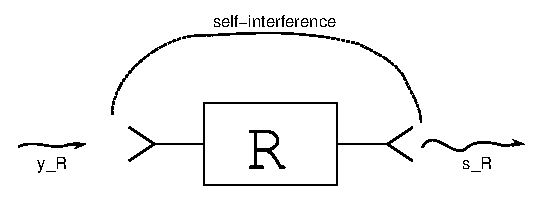
\includegraphics[scale=1]{Relay_self_interference}	
			\caption{Relay with self-interference}
			\label{fig:relay_self_interference}
		\end{figure}	
	\item[$\rightarrow$] Full\,-\,duplex relays are difficult to implement. The design of full\,-\,duplex relays is an active area of research.
	\item[$\rightarrow$] Majority of existing literature assumes half\,-\,duplex relaying.
\end{itemize}
\paragraph{Half\,-\,duplex relaying:} 
R transmits and receives in different time slots and/\,or different frequency bands. Typically, a two\,-\,phase protocoll is used:
\begin{itemize}
	\item[] \textbf{Phase 1}: S transmits, R and D receive 
	\begin{figure}[ht]
		\centering
		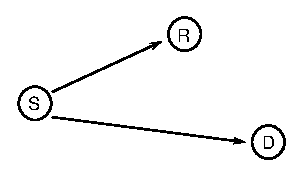
\includegraphics[scale=1.3]{Relay_HalfDuplex_1}	
		\caption{Half-duplex Relaying: Phase 1}
		\label{fig:relay_halfduplex_1}
	\end{figure}
	\item[] \textbf{Phase 2}: R transmits, D receives, S may or may not transmit 
	\begin{figure}[ht]
		\centering
		\includegraphics[scale=1.3]{Relay_HalfDuplex_2}	
		\caption{Half-duplex Relaying: Phase 2}
		\label{fig:relay_halfduplex_2}
	\end{figure}
\end{itemize}
There are different relaying strategies that differ in the processing applied at the relay. The most popular are:
\begin{itemize}
	\item Decode\,-\,and\,-\,Forward
	\item Amplify\,-\,and\,-\,Forward
	\item (Compress\,-\,and\,-\,Forward)
\end{itemize}

\subsubsection{Decode\,-\,and\,-\,Forward (DF) Relaying}
In DF relaying, the relay detects and decodes the signal received from the source before encoding it and  forwarding it to the destination.
	\begin{figure}[ht]
		\centering
		\psfrag{h_SR}[bl][bl][1]{$h_{SR}$}
		\psfrag{h_RD}[bl][bl][1]{$h_{RD}$}
		\psfrag{h_SD}[bl][bl][1]{$h_{SD}$}
		\psfrag{y_R}[bl][bl][1]{$y_R$}
		\psfrag{y_D1}[bl][bl][1]{$y_{D,1}$}
		\psfrag{y_D2}[bl][bl][1]{$y_{D,2}$}
		\psfrag{x_R}[bl][bl][1]{$x_R$}		
		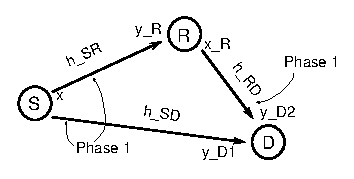
\includegraphics[scale=2]{DF_Relaying}	
		\caption{Decode\,-\,and\,-\,forward Relaying}
		\label{fig:df_relaying}
	\end{figure}
\paragraph{Phase 1:}
\begin{itemize}
	\item R receives: $ y_R = h_{SR}x + n_R $
	\item D receives: $ y_{D1} = h_{SD}x + n_{D1} $
	\item with: 
	\begin{itemize}
		\item transmit signal $x, \mathcal{E}_s = \mathcal{E}\{|x|^2\} $
		\item AWGN $n_R $ and $ n_{D1}$, $\sigma_n^2 = \mathcal{E}\{|n_R|^2\} = \mathcal{E}\{|n_{D1}|^2\} $
	\end{itemize}
\end{itemize}
\paragraph{Phase 2:}
\begin{itemize}
	\item R decodes and forwards $x_R$ (estimate of $x$)
	\item D receives: $ y_{D2} = h_{RD}x_R + n_{D2} $
	\begin{itemize}
		\item $x_R$ is estimate of $x $ after decoding at R
		\item $\sigma_n^2 = \mathcal{E}\{|n_{D2}|^2\}\,;\quad \mathcal{E}_R = \mathcal{E}\{|x_R|^2\} $
		\item weassume: S is silent in Phase 2		 
	\end{itemize}
\end{itemize}
\paragraph{}
\begin{itemize}
	\item The capacity at the three node relay channel is not known!
	\item We provide an achievable rate under the following simplifying assumption: The direct source\,-\,relay link is not used/\,exploited.
	\item Achievable rate without S\,-\,D link:
	\begin{align*}
		\boxed{C_{DF} = \frac{1}{2}\text{min}\bigl\{\log_2\bigl(1 + \frac{\mathcal{E}_S|h_{SR}|^2}{\sigma_n^2}\bigr),\,\log_2\bigl(1 + \frac{\mathcal{E}_R|h_{RD}|^2}{\sigma_n^2}\bigr)\bigr\} }	
	\end{align*}	 
	\begin{itemize}
		\item factor $\frac{1}{2} $ is due to the fact that we use two time slots to transmit one packet
		\item $\text{min}\{\ldots\} $ means we are limited by the weaker link (bottle\,-\,neck)
		\item If power allocation is possible, the total power $ \mathcal{E} = \mathcal{E}_S + \mathcal{E}_R $ should be divided between S and R to guarantee:
		\begin{align*}
			&\frac{\mathcal{E}_S|h_{SR}|^2}{\sigma_n^2} = \frac{\mathcal{E}_R|h_{RD}|^2}{\sigma_n^2},\\
			&\mathcal{E}_R = \frac{|h_{SR}|^2}{|h_{SR}|^2 + |h_{RD}|^2}\cdot\mathcal{E},\\
			&\mathcal{E}_S = \frac{|h_{RD}|^2}{|h_{SR}|^2 + |h_{RD}|^2}\cdot\mathcal{E}
		\end{align*}
	\end{itemize}
	\item Outage\,-\,probability in fading:
	\begin{itemize}
		\item We transmit with fixed rate R
		\item An outage occurs, if:
		\begin{align*}
			\frac{1}{2}\log_2\Bigl(1 + \underbrace{\frac{\mathcal{E}_S|h_{SR}|^2}{\sigma_n^2}}_{= \gamma_{SR}}\Bigr) &< R \quad	\text{or} \\
			\frac{1}{2}\log_2\Bigl(1 + \underbrace{\frac{\mathcal{E}_R|h_{RD}|^2}{\sigma_n^2}}_{= \gamma_{RD}}\Bigr) &< R
		\end{align*}
		\begin{align*}
			\boxed{\gamma_{SR} < \underbrace{2^{2R} - 1}_{\gamma_T} \quad \text{or}\quad \gamma_{RD} < 2^{2R} - 1}
		\end{align*}
	\end{itemize}
\end{itemize}


\end{document}				